%File: submission_v15.tex --- AAAI-27 anonymous submission (final; integrates the scale and external-map studies)
% "An Empirical Analysis of Transfer for Dynamic Path Planning"
% Built on the official AAAI-27 author kit (aaai2027.sty, TemplateVersion 2027.1).
\documentclass[letterpaper]{article} % DO NOT CHANGE THIS
\usepackage[submission]{aaai2027}  % DO NOT CHANGE THIS
\usepackage[hyphens]{url}  % DO NOT CHANGE THIS
\usepackage{graphicx} % DO NOT CHANGE THIS
\urlstyle{rm} % DO NOT CHANGE THIS
\def\UrlFont{\rm}  % DO NOT CHANGE THIS
\usepackage{natbib}  % DO NOT CHANGE THIS AND DO NOT ADD ANY OPTIONS TO IT
\usepackage{caption} % DO NOT CHANGE THIS AND DO NOT ADD ANY OPTIONS TO IT
\frenchspacing  % DO NOT CHANGE THIS
%
% Recommended for better-looking tables
\usepackage{booktabs}
\usepackage{amsmath}
%
\pdfinfo{
/TemplateVersion (2027.1)
}
\setcounter{secnumdepth}{0}

\usepackage{needspace}
% Float packing: allow taller bottom floats so single-column figures can
% sit at page bottoms instead of bisecting straddling paragraphs.
\renewcommand{\bottomfraction}{0.6}
\renewcommand{\topfraction}{0.9}
\renewcommand{\textfraction}{0.07}

% Custom macros

\title{An Empirical Analysis of Transfer for Dynamic Path Planning}
\author{
    Anonymous Submission
}
\affiliations{
}

\begin{document}

\maketitle

\begin{abstract}
We study the dynamic path planning problem, where an agent plans a route among moving obstacles, and ask whether heuristics learned on training maps transfer to unseen environments, zero-shot or from a few labeled target maps. Within budgeted time-expanded A\textsuperscript{*}, and with the right training formulation and planner integration, a single learned heuristic transfers zero-shot to new maps drawn from six procedural continuous dynamic suites. It was selected on development maps, frozen before the confirmation maps were generated, and given no future-motion input (the planner retains the exact obstacle trajectories). Yet it improves success over a geometric anchor while expanding 73--95\% fewer nodes on maps both methods solve. Applied unchanged to roadmaps rebuilt at 192--2{,}048 nodes, it expands fewer nodes than the anchor on jointly solved maps in every estimable case, and a preregistered GPU wall-time crossover against tuned weighted A\textsuperscript{*} is met on spiral at 512 nodes. In a descriptive map-level analysis of 21 held-out MovingAI-derived maps, it improves success over the anchor but stays behind tuned weighted A\textsuperscript{*}; few-shot adaptation improves unseen street maps; no gain is detected on dungeon maps. Selected discrete-grid experiments show a smaller, rank-only effect. In static few-shot experiments with one labeled target map, low-rank adaptation preserves success better than full fine-tuning; with sixteen maps, full fine-tuning searches more efficiently at similar success. In a matched-label factorial, full fine-tuning and from-scratch training degrade when a fixed label count is drawn from very few distinct worlds; spreading that count across more worlds prevents the degradation in the tested cells. No architecture is uniformly best across the tested formulations: MLPs, recurrent models, Hierarchical Reasoning Models, and U-Nets each lead in different settings, and hierarchy-specific gains do not persist.
\end{abstract}

\section{Introduction}

Dynamic path planning searches over both configuration and time: when obstacles move, a planner must consider waiting, detouring, and timing, and the search space grows accordingly \citep{silver2005cooperative,phillips2011sipp}. The geometric admissible heuristics that make A\textsuperscript{*} \citep{hart1968astar} efficient on static maps (the \emph{anchor} baselines of this paper) ignore exactly these temporal effects, so search effort grows sharply with moving obstacles. Learned heuristics can reduce search effort \citep{arfaee2011bootstrap,bhardwaj2017sail,yonetani2021neuralastar}, but a deployed planner benefits only if a trained heuristic remains useful on maps it has never seen. We study zero-shot and few-shot transfer of learned heuristics to unseen environments for dynamic path planning. Budgeted time-expanded A\textsuperscript{*} serves throughout as a controlled measurement substrate; we do not propose it as a replacement for dedicated dynamic planners.

We organize the experiments around three factors: the training formulation, the way the prediction enters the planner, and the distribution of target supervision. Each factor is evaluated first on static suites, then under deterministic dynamics. Comparisons use matched controls throughout: aware/blind pairs (with and without future-motion input) matched apart from the channels' first-layer parameters, identical weights under different integrations, anchor-calibrated budgets, and map-level paired inference \citep{henderson2018matters,agarwal2021precipice,pineau2021reproducibility}. Confirmatory comparisons, units, and criteria are specified before test evaluation. Across the tested settings, the training formulation, planner integration, and supervision distribution explain the observed transfer outcomes more consistently than model family.

\begin{figure*}[t]
\centering
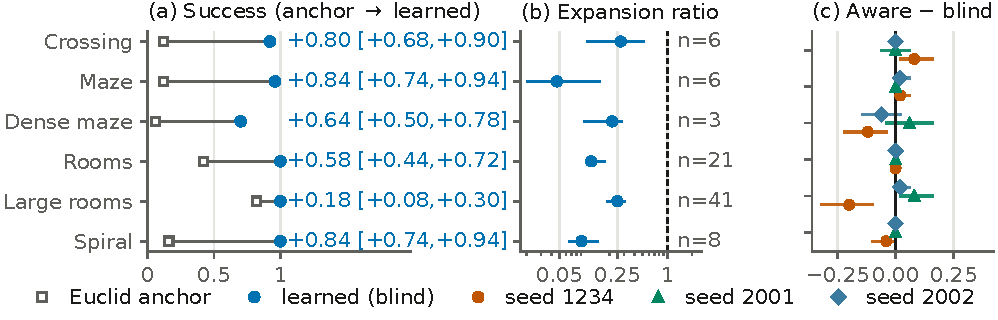
\includegraphics[width=0.98\textwidth]{figures/fig_dynamic_headline.pdf}
\caption{Dynamic zero-shot transfer of the fixed blind U-Net (no future-motion input) on the 50-map-per-suite confirmation cohort (held out from training: crossing, a distinct topology, and dense maze/large rooms, parameter/scale shifts; maze, rooms, spiral use trained generators, disjoint maps). (a) Anchor and learned success per suite; paired mean deltas (map-level 95\% CIs, all six excluding zero; marginal). (b) Matched-solved expansion ratios, conditional on joint success (log axis, 95\% CIs); $n$ = jointly solved count (dense maze $n{=}3$ descriptive). (c) Aware$-$blind success deltas, three pipelines, rows as in (a) (large rooms flips sign).}
\label{fig:dynamic}
\end{figure*}

Our contributions are:
\begin{itemize}
    \item \textbf{Dynamic zero-shot transfer with one fixed learned heuristic.} A single U-Net heuristic improves success on all six dynamic suites of a 50-map-per-suite confirmation cohort ($+0.18$ to $+0.84$) and cuts matched expansions by 73--95\% on jointly solved maps. Every paired map-level CI excludes zero and every exact McNemar test survives BH correction. The model was development-selected, frozen before the confirmation cohort was generated, and given no future-motion input. Three suites are held out from training: one distinct topology and two parameter/scale shifts; the remaining three draw disjoint maps from trained families. The expansion advantage persists in every estimable cell up to 2{,}048 nodes. Descriptively at map level, it beats the anchor, though not tuned weighted A\textsuperscript{*}, on 21 held-out MovingAI-derived maps.
    \Needspace{2\baselineskip}
    \item \textbf{Training formulation and planner integration determine whether transferred predictions reduce search.} Changing the coupled input--target--output formulation yields useful recurrent-model guidance where the scalar formulation collapses; changing only the planner integration makes an inert discrete residual useful; and sharing one search state turns an exact oracle from a six-map loss into a six-map win. A negative planning result therefore does not isolate the model unless target and search interface are held fixed.
    \item \textbf{At fixed label count, distinct-world coverage controls the observed held-out degradation in the tested matched-label factorial.} With scarce static supervision, low-rank adaptation preserves the transferred prior while full fine-tuning is unstable; with more supervision, full fine-tuning often overtakes it on search effort at near-parity success. The largest held-out losses occur for full fine-tuning and from-scratch training when a fixed label count comes from very few distinct worlds; spreading the same labels across more worlds prevents those losses in the tested cells, and targeted redraws preserve the positive direction. Low-rank adaptation degrades least often, though one redraw LoRA cell has a harmful interval excluding zero.
\end{itemize}
Weighted A\textsuperscript{*}, SIPP, and an external MovingAI test bound the scope. Under the tested weighted-A\textsuperscript{*} grid, the learned heuristic keeps a success advantage only on spiral, with lower matched expansions on four suites and higher path cost on two. Unbudgeted safe-interval planning (SIPP) solves every instance feasible under the implemented collision model optimally. An initial five-map MovingAI-derived test is anchor-negative, but the result does not reproduce in a 21-map source-held-out follow-up; tuned weighted A\textsuperscript{*} stays stronger externally. Future-window inputs, adapter interpolation, and hierarchy-specific depth add no consistent value. A restricted-observation heuristic with one Bellman backup and frozen scale calibration beats a complete-map comparator on expansions.

\section{Problem Formulation and Learned-Heuristic Interfaces}

\textbf{Planning problems.} In the continuous setting, a point robot plans on a probabilistic roadmap \citep[PRM;][]{kavraki1996prm} built over a square world of side length $L{=}1.0$ ($2.0$ for the large-room family). Units are abstract. Each roadmap has 192 nodes (start, goal, and 190 sampled free-space nodes) with $k{=}7$ nearest-neighbor candidate edges per node (doubled for start and goal, then symmetrized; appendix). Edges are validated by sampled collision checks ($0.01L$ resolution); unconnected worlds are rejected. Static search states are roadmap nodes, edge costs are Euclidean lengths $\ell(e)$, and the anchor heuristic is Euclidean distance to the goal, $h_0(v) = \lVert x_v - x_g \rVert$.

In the dynamic setting, obstacles move on deterministic trajectories and the search state is a pair $(v,t)$ of node and discrete time step of duration $\Delta t$. The planner may traverse an edge, taking $\tau(e) = \lceil \ell(e) / (v_{\mathrm{agent}} \Delta t) \rceil$ steps ($v_{\mathrm{agent}}$: agent speed), or wait one step. Transitions are validated against the obstacle trajectories by collision checks sampled along the edge (moves) or across the time interval (waits). Cost is arrival time in steps; search runs to a horizon $t_{\max}$; and the anchor is the travel-time lower bound $h_0(v,t) = \lVert x_v - x_g \rVert / (v_{\mathrm{agent}} \Delta t)$, constant in $t$, so anchor and cost share units.

In the discrete setting, agents plan on occupancy grids of $20{\times}20$ to $256{\times}256$ cells with Manhattan distance as the anchor and an analogous capped residual target (appendix).

\textbf{Supervision targets.} The exact cost-to-go $h^{*}$ comes from graph Dijkstra on the static roadmap and from backward space--time Dijkstra over $(v,t)$ dynamically. The regression target is the normalized anchor residual $\bar\delta^{*}(s) = \mathrm{clip}\!\left(h^{*}(s) - h_0(s),\, 0,\, c\,T\right)/T$. Here $T$ is the normalization scale: $T{=}L$ statically, and dynamically $T = L/(v_{\mathrm{agent}}\Delta t)$, the map-crossing time in steps, identical across dynamic suites by construction. The cap $c{=}4.0$ is in normalized units, and unreachable states are masked from the loss. Scalar models predict $\bar\delta_\theta$ from per-node feature tokens. Field models map an eight-channel input raster (appendix) to a goal-conditioned residual raster sampled at node positions. At integration the prediction is rescaled: $\hat h_\theta(s) = h_0(s) + T \cdot \mathrm{clip}(\bar\delta_\theta(s), 0, c)$.

\textbf{Planner integrations.} Under \emph{additive} integration the planner orders states by $f(s) = g(s) + \hat h_\theta(s)$, sacrificing admissibility for guidance. Empirical path-cost ratios are reported wherever additive integration is used. The classical control is weighted A\textsuperscript{*} \citep{pohl1970}, which orders states by $f(s) = g(s) + w_h\, h_0(s)$ with a per-suite success-tuned inflation $w_h$. Under \emph{focal (rank-only)} integration \citep{pohl1970,pearl1982semiadmissible}, the anchor priority $f_0(s) = g(s) + h_0(s)$ defines the band $\mathrm{FOCAL}_w = \{ s \in \mathrm{OPEN} : f_0(s) \leq w \cdot \min_{u \in \mathrm{OPEN}} f_0(u) \}$, and the learned prediction orders expansions only within the band. At $w{=}1.0$ the learned score merely breaks ties among minimum-priority states, preserving the anchor's path-cost optimality when search completes (budgets can still change success).

In the restricted-observation study, one inference-time Bellman backup over a radius-bounded local subgraph turns learned exit values into the heuristic (scale calibrated once on a disjoint block).

\textbf{Transfer protocol.} Zero-shot transfer applies a trained-and-fixed heuristic to unseen maps (held-out suite distributions where applicable), with no target-label training or adaptation. Selecting the deployed heuristic (\emph{provider} selection), where it occurs, uses a disjoint development cohort and is disclosed. Few-shot adaptation draws $K$ labeled target maps and compares low-rank adaptation \citep[LoRA;][]{hu2021lora} (rank 8 for the HRM, rank 24 for the ON-LSTM's wider hidden layer), full fine-tuning, and training from scratch. LoRA and full fine-tuning start from the same trained checkpoint. Scratch uses the same architecture and schedule from random initialization.

\section{Experimental Setup}

\textbf{Environment families.} A \emph{family} is a procedural map generator; a \emph{suite} is a named evaluation condition; a \emph{world} is one sampled environment (interchangeably, a \emph{map}). Continuous worlds come from our procedural generator (specification tables in the appendix; code in the artifact archive). The static hard families are wall constructions---\emph{maze}/\emph{dense maze} (corridor mazes; the dense variant narrows gaps to $0.115L$), \emph{rooms}/\emph{large rooms} (partition walls with doorways; the large variant doubles the side length), \emph{spiral}, and \emph{bugtrap}. Static training uses the maze, rooms, and spiral families; dense maze, bugtrap, and large rooms are held out from training (bugtrap: distinct topology; dense maze/large rooms: gap- and scale-shifted variants of trained generators).

Dynamic suites add 3--5 moving circular obstacles (\emph{patrollers}) per world that sweep line segments with triangle-wave motion (radius 0.055--0.080$L$, span 0.36--0.50$L$, period 0.14--0.30 of the horizon; appendix). A \emph{crossing} open-arena suite serves as a timing control. \emph{Dynamic training draws worlds only from the dynamic maze, rooms, and spiral families; dynamic dense maze, crossing, and large rooms are held out}: crossing is a distinct open-arena topology; dense maze narrows corridors and adjusts patrollers; large rooms doubles the scale and speeds the agent. No learned model observes a test world during training. Evaluation cohorts come from disjoint seed ranges, checked by world fingerprints.

\textbf{Models.} Scalar models consume per-node token sequences (62 tokens $\times$ 16 dims; appendix) and include an MLP, an LSTM \citep{hochreiter1997lstm}, an ON-LSTM \citep{shen2019onlstm}, and a Hierarchical Reasoning Model \citep[HRM;][]{wang2025hrm} with an adaptive-computation port \citep{graves2016act,banino2021pondernet}. Field models consume the eight-channel $64{\times}64$ raster and include a FiLM-conditioned U-Net \citep{ronneberger2015unet,perez2018film}, a field HRM, and a field ON-LSTM (parameters in the appendix). Dynamic variants append $W$ future-occupancy channels ($W{=}8$ aware = ground-truth occupancy at the next eight steps; $W{=}0$ blind). Unless a specific experiment states otherwise, the continuous residual models share one AdamW recipe on a smooth-L1 loss over the capped normalized residual (optimizer constants and architecture tables in the appendix; complete constructors in the artifact). Within each direct architecture comparison, models are trained under one matched recipe on identical data.

\begin{table*}[t]
\centering
\small
\begin{tabular}{lcccccc}
\toprule
Suite & $w_h$ & Success learned & Success WA* & Expansions learned/WA* [95\% CI] ($n$) & Subopt.\ learned & Subopt.\ WA* \\
\midrule
Crossing & 1.5 & 0.92 & 1.00 & 0.825 [0.531, 1.167] (46) & 1.164 & 1.008 \\
Maze & 5 & 0.96 & 0.96 & 0.601 [0.440, 0.835] (47) & 1.013 & 1.017 \\
Dense maze & 5 & 0.70 & 0.70 & 0.982 [0.823, 1.089] (34) & 1.008 & 1.006 \\
Rooms & 3 & 1.00 & 0.98 & 0.554 [0.439, 0.798] (49) & 1.019 & 1.015 \\
Large rooms & 1.5 & 1.00 & 0.98 & 0.728 [0.536, 0.966] (49) & 1.083 & 1.003 \\
Spiral & 5 & \textbf{1.00} & 0.70 & 0.217 [0.183, 0.312] (35) & 1.014 & 1.013 \\
\bottomrule
\end{tabular}
\caption{Fixed learned heuristic versus per-suite success-tuned weighted A\textsuperscript{*} (original grid), confirmation cohort at binding budgets. Expansions: median learned-to-weighted ratio on the $n$ jointly solved maps [map-bootstrap 95\% CI]. Subopt.: mean arrival over optimal on the same maps (paired intervals in text). Bold: the only BH-significant success difference ($q{=}3.7\times10^{-4}$; crossing's four-map gap $q{=}0.375$).}
\label{tab:wastar-main}
\end{table*}

\textbf{Evaluation.} Each suite is evaluated at an expansion budget from anchor-only calibration: the fixed-grid budget whose anchor success is closest to pre-specified targets (evenly spaced in $[0.45,0.70]$; ties to the smaller budget), chosen before any learned method is compared. The smallest selected budget is the \emph{binding} budget, the primary operating point. The coarse budget grid means realized anchor success at calibration can fall outside the target band (0.05--0.75 dynamic, 0.25--0.62 static; rates in the appendix). Static calibration shares worlds with evaluation (anchor-only; disclosed limitation). The dynamic 50-map-per-suite cohort and the 144-map restricted-observation cohort are \emph{confirmation} cohorts: their budgets were frozen before the cohorts were generated.

Success means reaching the goal within budget; appendix success-vs-budget curves up to $4\times$ binding mitigate single-threshold dependence. Search effort is the \emph{matched-solved expansion ratio}: the median over jointly solved maps of the per-map ratio of learned to anchor expansions. Because it conditions on joint success, it can favor methods that solve only easier maps. Success is therefore reported first, with path-cost ratios reported separately (appendix).

\textbf{Statistics.} \looseness=-1 Success comparisons use paired McNemar tests with Benjamini--Hochberg correction within each experiment's set of suites (adjusted values reported as $q$). Interval estimates are percentile bootstraps (10{,}000 resamples) whose resampling unit is the evaluation map; repeated adaptation or model seeds are averaged within maps before resampling; intervals reflect map uncertainty conditional on the evaluated seeds. Per-suite bootstrap intervals (Figure~\ref{fig:dynamic}) are marginal. The corrected McNemar tests are primary (full policy in the appendix).

Method-versus-method claims use direct paired contrasts. Unless noted, continuous experiments use one primary training seed; the dynamic result adds two retrained pipelines.

\section{Dynamic Zero-Shot Transfer}

\textbf{Setting and fixed-model protocol.} The dynamic experiment trains on the dynamic maze, rooms, and spiral families and evaluates on all six dynamic suites---three sharing a training generator (disjoint maps) and three held out as above (dense maze, crossing, large rooms). The training run keeps 53 usable worlds of 72 candidates (24 per family; rules and label counts in the appendix). The original 20-map-per-suite cohort served as \emph{development} data: on it we selected the field U-Net \emph{blind} twin and froze its checkpoint, the additive integration, and the per-suite budgets. The 50-map-per-suite \emph{confirmation} cohort was then generated from a pre-specified seed range, map-disjoint by fingerprint check, with no further choices. Selection still happened, on development data, and the protocol protects only the confirmation cohort. The planner and collision checker always use the true trajectories when validating $(v,t)$ transitions, so the aware/blind ablation changes only the heuristic's input.

\textbf{Confirmation result.} On the confirmation cohort, the fixed blind U-Net raises success on all six suites: deltas $+0.18$ to $+0.84$, every paired map-level 95\% CI excluding zero (exact McNemar $q \leq 0.0039$; every discordant map favors the learned heuristic). Matched expansion-ratio medians are 0.047--0.273, a 73--95\% effort reduction on jointly solved maps (Figure~\ref{fig:dynamic}; $n$ 3--41). On jointly solved maps the anchor's paths are optimal (admissible anchor; verified), and learned mean suboptimality spans 1.000--1.216 per suite, largest on crossing (anchor-joint maps; the control table's joint sets differ; appendix). Gains on the three held-out suites ($+0.80$ crossing, $+0.64$ dense maze, $+0.18$ large rooms) show transfer under topology and parameter/scale shift.

\textbf{Independent retraining robustness.} Two additional full training pipelines with independent seeds (2001, 2002) reproduce the success pattern on the same confirmation cohort. They used a larger world-collection budget (139 and 149 usable worlds versus 53; appendix): seed and data scale vary together. Across the three pipelines, 17 of 18 pipeline--suite paired CIs exclude zero (deltas $+0.10$ to $+0.88$; the exception is a near-ceiling large-rooms cell). Effort magnitudes are pipeline-stable on three suites (0.047--0.135) and pipeline-variable on three (0.216--0.625). The retrained models are evaluated on the same 50 maps (retraining robustness, not cohort replication).

\textbf{Graph scale and wall time.} On shared fresh worlds connectable at every tested density (192--2{,}048 nodes, rebuilt per size; appendix), every estimable learned-to-anchor expansion-ratio interval (defined on jointly solved maps) is below one (medians 0.06--0.29). Under the frozen scaled calibration, the preregistered success-breadth criterion passes at 192 and 512 nodes and fails at 1{,}024 and 2{,}048 through floor/ceiling operating points; no estimable cell reverses. A post-hoc sensitivity pass at discriminative budgets resolves four of seven degenerate cells in the learned arm's favor without changing frozen verdicts. Estimated learned wall-time slopes are lower than the anchor's and tuned weighted A\textsuperscript{*}'s on every non-degenerate suite (slope-contrast CIs exclude zero; SIPP under its own protocol), and a preregistered GPU wall-time crossover criterion is first met on spiral at 512 nodes and holds at 1{,}024 (BH $q{=}0.0002$ across the 24-cell scan). The other five suites do not cross by 2{,}048 (appendix).

\textbf{Tuned weighted A\textsuperscript{*} control.} Because the anchor is deliberately simple, we also compare against per-suite success-tuned weighted A\textsuperscript{*} (grid $w_h \in \{1.1, 1.2, 1.5, 2, 3, 5\}$; frozen rule; tuned on development data only, after the learned results were known; one confirmation evaluation; appendix). The comparison yields a three-way tradeoff, not dominance (Table~\ref{tab:wastar-main}). \emph{Success:} no BH-corrected difference on five suites (crossing's four-map weighted advantage has $q{=}0.375$). The learned heuristic holds the one BH-significant advantage, on spiral ($+0.30$ $[+0.18,+0.42]$; 15/0 discordant). \emph{Effort:} learned-to-weighted medians are below parity everywhere (0.217--0.728), with marginal intervals excluding parity on four of six suites (descriptive---corrected success tests carry the inference). \emph{Path quality:} the additive heuristic pays premiums over tuned inflation on crossing ($+0.156$ $[+0.116,+0.200]$) and large rooms ($+0.080$ $[+0.058,+0.105]$); the other four suites stay within $\pm 0.005$, intervals covering zero.

A disclosed post-hoc grid extension to $w_h \in \{7, 10\}$ changes no inferential conclusion; dense maze re-selects $w_h{=}7$ with point-estimate shifts only (0.74 vs.\ 0.70, exact $p \geq 0.5$; appendix).

\textbf{Unbudgeted SIPP reaches the feasibility ceiling.} Discrete-time SIPP \citep{phillips2011sipp} on the identical substrate, validated by a precommitted outcome-agreement check against backward space--time Dijkstra on all 300 confirmation instances, solves every feasible instance optimally under the implemented collision model; its per-suite success (0.94--1.00) equals the substrate's feasibility ceiling. It uses interval states and a different resource unit, so it serves as an optimal boundary rather than a budget-matched competitor; the learned result concerns budgeted time-expanded search (wall times and tables in the appendix).

\textbf{External-geometry boundary.} MovingAI maps \citep{sturtevant2012movingai} are converted to the canonical substrate (64$\times$64 majority-coarsened occupancy, rectangle-decomposed obstacles, trained maze-family patroller dynamics) and evaluated under the frozen calibration/tuning protocol. An initial five-map pilot found no anchor-relative success gain (instance-level tests nested in five maps); a residual probe associates the failure with degraded prediction on converted geometry (pilot and probe in the appendix). In a frozen source-map-level follow-up, the pilot's anchor-relative result does not reproduce: 37 of 40 selected maps yield usable instances, eight pool maps per category supply all labels and calibration, and the 21 held-out maps (12 street, 9 dungeon) each contribute one map-level aggregate over 12 frozen instances.

Zero-shot (descriptive, map level), the frozen heuristic beats the anchor on both held-out groups (street $+0.10$ $[+0.04,+0.16]$, dungeon $+0.20$ $[+0.09,+0.32]$); tuned weighted A\textsuperscript{*} stays stronger in success and matched effort on both. Within the repaired eight-test family, adapting on the eight pool street maps improves success on the twelve unseen street maps (BH $q \leq .035$ for low-rank and full fine-tuning); no held-out dungeon gain is detected, and the pilot's pool-map dungeon improvement does not generalize to held-out maps. The family's eight-versus-one coverage contrast---a post-outcome balanced correction of an unbalanced one-map schedule, not preregistered---is positive only for street full fine-tuning ($+0.037$, $q{=}.026$). At the matched 65{,}536-label budget from-scratch training has the highest observed street success: the study establishes transfer to unseen maps, not an advantage of the procedural source checkpoint (appendix).

\textbf{Future-window inputs provide no consistent benefit.} The primary model is already the blind twin; the aware twin adds the eight future-occupancy input channels (first layer only; otherwise matched). On the confirmation cohort the contrast is suite-dependent in both directions and unstable across pipelines. Across 18 contrasts, each twin's paired intervals exclude zero twice, never in the same suite and direction across pipelines (large rooms flips sign). The canonical pipeline trained on fewer worlds, but the two collection-matched retrains still disagree (Figure~\ref{fig:dynamic}(c); appendix). After full fine-tuning at $K{=}16$, eight of nine aware$-$blind differences are non-positive (the ninth includes zero; appendix). We report a failure to observe a systematic future-window benefit under deterministic dynamics---not equivalence, and not harm. Stochastic motion is untested.

\section{Effects of Supervision Target and Planner Integration}

\textbf{Static family transfer.} On the six calibrated static suites, the transferred field HRM reaches success 0.75--1.00 against the anchor's 0.25--0.58 (BH-adjusted $q \leq 0.025$ on four suites; on the other two, only other learned arms reach corrected significance; matched ratios 0.521--0.850; appendix). Three of six suites are held out from training as above, and models trained on data pooled across the three source families (\emph{pooled} models) improve success on every held-out suite before any target labels are used.

\textbf{Supervised target.} On the calibrated hard static maps, a pooled ON-LSTM scalar residual model raises hard-maze success from 0.525 to 1.000 over the anchor ($q=4.3\times10^{-11}$). The scalar HRM, under the same recipe and data, instead collapses to a constant prediction at the residual cap and merely matches the baseline (the collapse reproduces under retuning; appendix). Retaining the HRM while changing input, target, and output head to the raster residual field raises hard-maze success from the run's anchor value 0.625 to 0.975 ($q=3.4\times10^{-4}$). A later run shows a well-trained scalar HRM is viable (ratios 0.427--0.822). The failure is therefore formulation-specific rather than intrinsic to the HRM. The field intervention changes input, target, and output head together, so it does not isolate which component matters.

\textbf{Planner integration.} The preferred integration differs between the two tested substrates. On continuous roadmaps, additive residuals exploit the gap the Euclidean anchor leaves (the field-HRM ratios above, at empirical path-cost ratios of roughly 1.02--1.14), while rank-only variants stay closer to plain anchor search. On discrete grids the learned signal is accurate: the pooled residual correlates 0.987--0.994 with the true residual across map sizes. But its magnitude fails to track scale (predicted/true mean falls 0.73 to 0.19 as maps grow), and every additive arm in a 22-suite transfer evaluation (appendix) is at or below its matched baseline. We then reuse the \emph{same} trained predictions only to rank expansions inside a $w{=}1.0$ focal band: expansions fall 6--15\% with no observed success regression \citep{chrestien2023rank}. Changing only the integration recovered the ordering signal. We interpret the cross-substrate pattern (additive helps against a looser anchor, ranking against a tighter one) as a supported hypothesis. Anchor tightness itself is not directly measured.

\textbf{Oracle integration control.} An oracle control removes model-estimation error: exact optimal values rank expansions inside a $w{=}1.10$ focal band against a matched focal baseline (129.7 expansions, six development maps). A second bound-certifying search that discards the main search's queue loses all six comparisons (141.2 expansions); reusing one queue and $g$-values wins all six (122.8). Because the values are identical, the comparison isolates search-state reuse (a development test).

\section{Few-Shot Adaptation}

\begin{figure}[b]
\centering
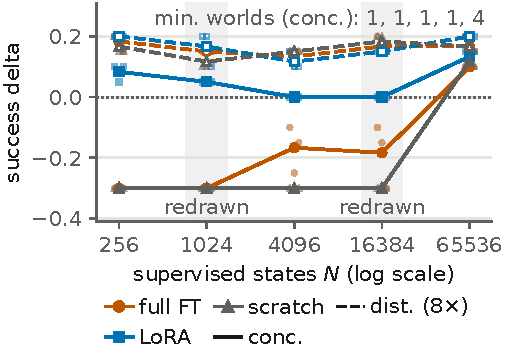
\includegraphics[width=0.98\columnwidth]{figures/fig_c14_dynamic.pdf}
\caption{The matched-label factorial, dynamic substrate (static panel and tables in the appendix): success delta vs.\ the frozen zero-shot source at fixed state count $N$, frozen test cohort, binding budgets. Solid: concentrated (fewest worlds supplying $N$; counts annotated); dashed: the same $N$ over $8\times$ as many worlds; small markers: the three adaptation seeds. Concentrated supervision drops held-out success for full fine-tuning and scratch; distributing the same labels prevents it. Shaded bands: $N$ levels with independent world redraws (positive contrasts preserved; one LoRA cell degrades; appendix).}
\label{fig:factorial}
\end{figure}

\textbf{Direct contrasts: LoRA retains success at $K{=}1$; full fine-tuning overtakes on effort by $K{=}16$.} At $K{=}1$ the map-paired full-FT$-$LoRA success difference is negative in all six cells (three held-out static targets $\times$ two backbones, HRM and ON-LSTM), with the 95\% interval excluding zero in four (appendix). LoRA retains the zero-shot gain (dense maze ratio 0.686, success $+0.467$); full fine-tuning reaches ratio 1.293 on large rooms, and scratch is harmful on dense maze ($-0.167$, interval excluding zero). At $K{=}16$ the contrast reverses on effort: the paired expansion-ratio difference favors full fine-tuning in all six cells, with the map-bootstrap interval excluding zero in five (up to $-0.366$ $[-0.489,-0.235]$). Success is at near-parity (one cell's interval favors full fine-tuning). A 27-cell matched-compute ablation finds bounded and unbounded LoRA nearly identical, so the output clamp does not explain why LoRA's effort gains stall at higher $K$ (appendix). LoRA is not universally protective (bugtrap ratio 1.153 by $K{=}32$). Dynamic maps are label-dense ($\sim$15{,}507 supervised states per world); at dynamic $K{=}1$ full fine-tuning does not collapse, and LoRA improves on the source rather than merely preserving it. Per-cell contrasts and $K$-indexed curves are in the appendix.

\textbf{A matched-label factorial separates label count from distinct-world coverage.} The $K$-indexed protocol confounds two quantities: adding maps adds labels and worlds together. A preregistered factorial therefore holds the number of supervised states $N$ fixed (256 to 65{,}536 by factors of 4) and varies only whether those states come from the fewest worlds that can supply them (\emph{concentrated}) or from eight times as many (\emph{distributed}). Both domains run matched optimizer steps, each cell adapting one deterministically sampled world set (seeds vary initialization and batch order; Figure~\ref{fig:factorial}; protocol and tables in the appendix). The preregistered primary hypothesis (a full-fine-tuning$\times\log N$ effort crossover) is rejected (interaction $-0.0025$ $[-0.0087, +0.0028]$). The coverage readout below is the prespecified secondary endpoint. Concentrated supervision causes a held-out success drop for full fine-tuning and scratch in both domains: $-0.300$ in every seed at dynamic concentrated $N \leq 1{,}024$, still negative in every seed at $N{=}16{,}384$ from one world (one seed excludes zero). Distributing the \emph{same} states across more worlds prevents the drop ($+0.15$ to $+0.20$; Figure~\ref{fig:factorial}).

The 30 direct distributed$-$concentrated contrasts (each pairing two of the 60 cells) receive BH-corrected sign-flip tests (post hoc, during review response; appendix). For full fine-tuning and scratch, $q{<}0.05$ in all 10 cells where concentration forces at most two distinct worlds and in none of the 10 where it forces four or more (threshold descriptive). In the original 60 cells, no LoRA interval excludes zero in the harmful direction (worst $-0.067$ $[-0.167, 0.000]$). Absent a noninferiority margin, this is a failure to observe degradation, not equivalence. Targeted world redraws preserve the coverage effect's direction (all 18 contrasts positive; scratch excludes zero in six, full fine-tuning in five); one redraw LoRA cell degrades with its interval excluding zero (still the least-degraded method in that cell; appendix). On the static matched ratios (the domain with adequate joint counts), full fine-tuning is at or below LoRA at every tested $N$, consistent with the rejected interaction; dynamic effort cells contain one jointly solved map and support no inference. Because ratios condition on solved maps, degraded-success cells can look spuriously efficient. The factorial's conclusions therefore rest on success. Within this factorial, low-rank adaptation's low-supervision advantage appears in \emph{success} and aligns with distinct-world coverage rather than label count.

\section{Scope and Boundary Results}

\textbf{Discrete transfer.} In a separate pooled-multitask study, the pooled HRM base under additive integration improves mean grid success over the Manhattan baseline (0.591$\to$0.612) at lower mean expansions (descriptive; appendix).

\textbf{Architecture and hierarchical depth.} Architecture rankings are task- and representation-dependent (the U-Net leads the dynamic field study, the ON-LSTM the early scalar stage). In compositional \emph{mission} tasks with oracle-verified headroom for deeper reasoning, no structured model meets the preregistered depth dose--response criterion, learned halting moves \emph{opposite} to the depth hypothesis, and constant-prediction collapse cells are excluded from capacity conclusions (statistics in the appendix). Follow-ups on persistent memory, iterative refinement, hierarchical substitution, and persistent search state are also negative (appendix). These negatives are formulation-specific; they do not show that recurrence, memory, or hierarchy are universally ineffective \citep{jolicoeur2025trm,czechowski2021subgoal}.

\textbf{Restricted-observation transfer.} A final static study restricts the model to a radius-0.20 local subgraph, trains it from behavior-derived returns, and integrates it through one inference-time Bellman backup with frozen scale calibration. On a disjoint 144-map confirmation cohort the local MLP reduces mean per-map expansions against the complete-map field HRM (difference $-12.96$, 95\% CI $[-16.30,-9.74]$) at matched empirical path quality; a separate control ranking within a $w{=}1.10$ focal band satisfies its bounded-suboptimality certificate on all 144 maps.\looseness=-1 The confirmation's path-quality criterion is comparator-relative, adopted after the absolute ceiling failed in development (ablations, per-suite table, timing in the appendix).
\section{Related Work}

\looseness=-1 \textbf{Learned guidance for search.} Learned heuristics arise from bootstrapping \citep{arfaee2011bootstrap}, oracle imitation \citep{bhardwaj2017sail}, differentiable search \citep{yonetani2021neuralastar}, grid transformers \citep{kirilenko2023transpath}, planning objectives \citep{ferber2020neural}, and ranking \citep{chrestien2023rank}. We retain classical graph search throughout, evaluating cross-family and dynamic transfer of identical models and additive-versus-rank-only integration of the \emph{same} predictions under one planner and information set \citep{pohl1970,pearl1982semiadmissible,aine2016mha}.

\looseness=-1 \textbf{Dynamic, real-time, and motion planning.} The dynamic substrate uses time-expanded search in the spirit of cooperative A\textsuperscript{*} \citep{silver2005cooperative}; safe-interval planning \citep{phillips2011sipp} is evaluated as an unbudgeted optimal control. The restricted-observation study relates to real-time heuristic search \citep{korf1990rta,koenig2006rtaa}; its one-step backup resembles a value-iteration-network update \citep{tamar2016vin,lee2018gppn} and neural algorithm execution \citep{velickovic2021nar} but runs once at inference on a radius-bounded subgraph. Learned samplers and end-to-end motion planners \citep{ichter2018sampling,qureshi2019mpnet} replace the planner itself; we keep the classical planner and learn only its guidance on a PRM \citep{kavraki1996prm}.

\looseness=-1 \textbf{Adaptation and recursive architectures.}\hspace{0.25em}LoRA \citep{hu2021lora}, model soups \citep{wortsman2022soups}, and task arithmetic \citep{ilharco2022task} motivate the low-rank and adapter-interpolation studies (appendix); the contribution is the low-rank-versus-full-rank comparison across label availability and supervision distribution. HRM \citep{wang2025hrm}, adaptive computation \citep{graves2016act,banino2021pondernet}, and simplified recursive models \citep{jolicoeur2025trm} motivate the architecture experiments; our results concern heuristic regression and integration, not their benchmarks.

\section{Limitations}

\looseness=-1 \textbf{Design and selection.} Most continuous primary results use one training seed; several stages reuse trained bases or test maps. In the original program the 50-map dynamic and 144-map restricted-observation cohorts are the protected confirmations (post-development; static calibration shares evaluation worlds); the scale study evaluates a fresh shared cohort after per-size calibration; the external study holds out 21 maps under pool-only calibration. Baselines are the anchor, weighted A\textsuperscript{*}, and SIPP; no external \emph{learned} planner is compared. A suite-indexing defect made four control runs evaluate \emph{sibling} cohorts (same-generator, unintended seeds); all were re-run on the frozen cohort under unchanged rules, identity hash-verified (appendix erratum; weighted A\textsuperscript{*} was unaffected).

\looseness=-1 \textbf{Statistics and coverage.} Matched-effort magnitudes vary by pipeline on three suites; quoted intervals underrepresent training-run uncertainty (ranges reported); the discrete result covers selected cells. Where original analyses pooled repeated evaluations, map-clustered reanalysis (appendix) supports the quoted conclusions (not every table regenerated). The factorial covers one target family per domain, three adaptation seeds, and one world set per cell (targeted redraws in the appendix); coverage counts worlds, not geometric diversity. Matching covers labels and steps, not world-generation cost. Per-cell readouts are marginal (adjusted inference covers the 30 contrasts; the threshold is descriptive). The five-map probe and its adaptation follow-up are post hoc; the map-scale study is a separate frozen design. The primary 192-node result is expansion-based (CPU timing sample in the appendix); the scale study measures wall time directly.

\looseness=-1 \textbf{Scope.} The restricted-observation confirmation is static, uses one seed and cohort, tests input restriction only, lacks a formal bound on the primary comparison, and is slower in wall time. Dynamic obstacles are deterministic; stochastic motion, kinodynamic constraints, multi-agent coupling, physical robots, and non-2-D settings are untested. External tests coarsen and rectangle-decompose source maps and add synthetic dynamics; the map-scale study uses one frozen pool/held-out split and a post-outcome balanced coverage family. The scale study conditions on worlds connectable at all four densities (rebuilt, not nested); its breadth criterion fails at the two largest sizes through floor/ceiling cells. SIPP's interval unit is not resource-equivalent to $(v,t)$ expansions. The graph-scale and 40-map external studies close the program (frozen designs, dated amendments); runtime slopes come from four graph sizes (appendix). Negative results are failures to observe improvement under the tested protocols, not universal rejections.

\section{Conclusion}

\looseness=-1 Across the tested settings, formulation and integration explained outcomes more consistently than model family: a model collapses or transfers with its formulation; identical predictions help or fail with integration. A development-selected blind U-Net, frozen before confirmation, transferred zero-shot: success rose on all six suites and matched expansions fell 73--95\%. \looseness=-1 Within the procedural substrate this is learned guidance under budgeted search, not a faster dynamic planner: against weighted A\textsuperscript{*} the success advantage survives only on spiral, and SIPP solves all feasible instances optimally. At 192--2{,}048 nodes the anchor-relative expansion advantage persists in all estimable cells, with a preregistered wall-time crossover on spiral. The five-map pilot's anchor-negative result does not reproduce at 21-map scale; tuned weighted A\textsuperscript{*} stays stronger externally; adaptation improves success on held-out street maps (no detected dungeon gain). Distinct-world coverage separates adaptation methods: low-rank preserves success with few worlds, full fine-tuning matches success at lower effort with more maps (static $K{=}16$), and spreading fixed labels over more worlds prevents the concentrated losses.

\clearpage
\bibliography{references}

% AAAI-27 requires the reproducibility checklist to be uploaded separately
% in the designated submission field; it should not be included in this PDF.

\end{document}
